% *******************************************************************************
% * Copyright (c) 2008 by Elexis
% * All rights reserved. This document and the accompanying materials
% * are made available under the terms of the Eclipse Public License v1.0
% * which accompanies this distribution, and is available at
% * http://www.eclipse.org/legal/epl-v10.html
% *
% * Contributors:
% *    G. Weirich
% *
% *  $Id: anleitung.tex 2417 2007-05-21 04:35:34Z rgw_ch $
% *******************************************************************************

% !Mode:: "TeX:UTF-8" (encoding info for WinEdt)

\documentclass[a4paper]{scrartcl}
\usepackage{german}
\usepackage[utf8]{inputenc}

% Hier ein etwas skurriler Block, der dazu dient, die Unterschiede
% zwischen pdflatex und latex auszubügeln
% Grafiken müssen als png oder gif (für pdflatex) und als eps (für Latex)
% vorhanden sein. Die Endung kann man beim \includegraphics jeweils weglassen,
% das System nimmt je nach Renderer die geeignete Variante.

\usepackage[pdftex]{graphicx}
\DeclareGraphicsExtensions{.pdf,.jpg,.png}

\usepackage{floatflt}
\usepackage[]{hyperref}
\usepackage{color}
\begin{document}
\title{Universal-Laborimport für HL7-Dateien}
\author{Gerry Weirich}
\maketitle
\section{Einführung}
Dieses Plugin dient dazu, Laborwerte von Labors oder Geräten zu importieren, für die kein spezifisches Import-Plugin existiert, die aber Dateien im HL7-Format erzeugen können.

\medskip

Dieses Plugin benötigt Elexis 1.4.0 oder höher.

\section{Konfiguration}

Wenn Sie das Plugin korrekt installiert haben, dann erscheint unter \textsc{Datei-Einstellungen-Datenaustausch} eine Seite 'HL7 Dateien', wo Sie eingeben müssen, in welchem Verzeichnis Elexis nach Labordateien suchen soll.

\section{Anwendung}
Klicken Sie einfach auf den Import-Knopf in der Labor-View (\ref{fig:lab1}).

\begin{figure}
  % Requires \usepackage{graphicx}
  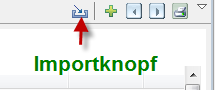
\includegraphics{abb1.png}\\
  \caption{Import starten}\label{fig:lab1}
\end{figure}


Nach dem Import werden alle heruntergeladenen Dateien in einem Unterordner 'archive' des Download-Verzeichnisses aufbewahrt, wo Sie sie nach einiger Zeit von Hand löschen können.

\end{document} 